\begin{frame}{$d(K^-, n \pi^+ \pi^-)"n"$ window selection}
  \begin{tabular}{cc}
    \begin{minipage}{0.5\hsize}
      \begin{figure}
        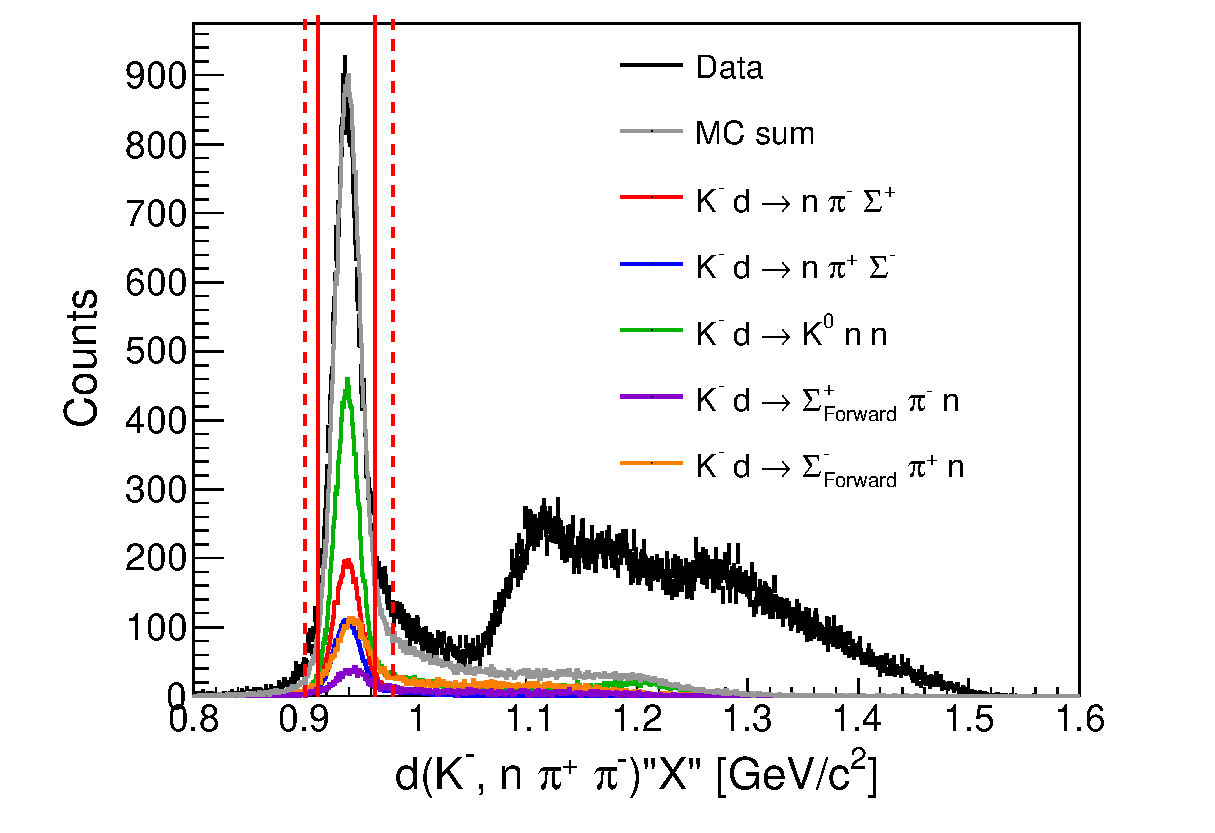
\includegraphics[width=5cm]{../pic/Run78/KN_reso/fitKNpipi_MM.eps}
      \end{figure}
    \end{minipage}

    \begin{minipage}{0.5\hsize}
      \begin{figure}
        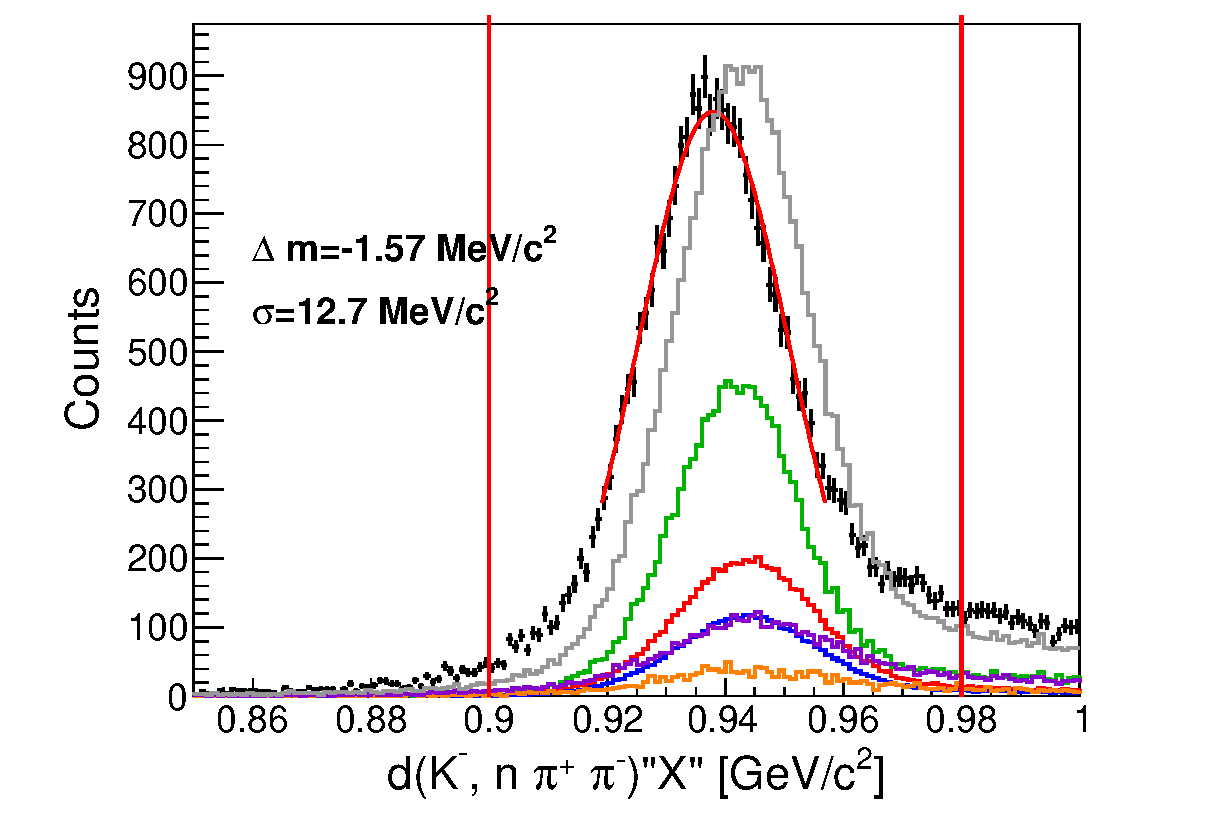
\includegraphics[width=5cm]{../pic/Run78/KN_reso/fitKNpipi_MM_fitData.eps}
      \end{figure}
    \end{minipage}
  \end{tabular}
  \vspace{5mm}\\
  \centering
  \small
  Right figure shows zoom up around $"n"$ region.\\
  Dotted line indicate before selection, solid line indicate $2\sigma$ selection.\\
  { \bf
    I chose $2\sigma$ selection to avoid tail components.
  }
\end{frame}
